% !TEX root = ../slides.tex
%%%%%%%%%%%%%%%%%%%%%%%%%%%%%%%%%%%%%%%%%%%%%%%%%%%%%%%%%%%%%%%%%%%%%%%%%%%%%%%%
% Session 4: The finite-element formalism
%%%%%%%%%%%%%%%%%%%%%%%%%%%%%%%%%%%%%%%%%%%%%%%%%%%%%%%%%%%%%%%%%%%%%%%%%%%%%%%%

\session{session04}{The finite-elements method}{The finite-element formalism}
{Sections 2.1--2.2}
{--}
{2.1--2.4}

\begin{frame}{Plan for today}
    \begin{enumerate}
        \item What is a finite element? Ciarlet's triplet $(K, \mathcal P, \mathcal N)$.
        \item Nodal basis and local interpolant.
        \item Reference elements and affine equivalence.
        \item Interpolation estimates: scaling arguments and the Bramble--Hilbert lemma.
    \end{enumerate}
    \bigskip
    \textbf{Motivation.} Céa's lemma reduces the error analysis to
    \[
        \inf_{v_h \in V_h} \|u - v_h\|_V \le \|u - \mathcal I_h u\|_V .
    \]
    We want a systematic way to build spaces $V_h$ (and interpolants $\mathcal I_h$) from \alert{local pieces}, and to estimate the interpolation error.
\end{frame}

\begin{frame}{The finite element}
    \begin{definition}[Finite element (Ciarlet)]
        A finite element is a triplet $(K, \mathcal P, \mathcal N)$ where
        \begin{enumerate}
            \item $K \subset \R^d$ is a bounded, simply connected open set with piece-wise smooth boundary (the \emph{element domain});
            \item $\mathcal P$ is a finite-dimensional space of functions on $K$ (the \emph{shape functions});
            \item $\mathcal N = \{N_1, \dots, N_N\}$ is a basis of $\mathcal P^*$ (the \emph{degrees of freedom}, or \emph{nodal functions}).
        \end{enumerate}
    \end{definition}
    \begin{itemize}
        \item Typical nodal functions: $N_i(v) = v(x_i)$, or $N_i(v) = \frac{\partial v}{\partial x_k}(x_i)$.
        \item They are usually defined on a larger space, e.g.\ $C^k(\overline K)$.
        \item If $x_i \in \partial K$ we need $\mathcal P \subset C^r(\overline K)$, and evaluate by limits.
        \item ``$\mathcal N$ is a basis of $\mathcal P^*$'' is also called \emph{$\mathcal P$-unisolvence}: $v \in \mathcal P$ and $N_i(v) = 0$ for all $i$ $\Rightarrow$ $v = 0$.
    \end{itemize}
\end{frame}

\begin{frame}{Nodal basis and local interpolant}
    \begin{definition}[Nodal basis]
        The nodal basis of $(K,\mathcal P,\mathcal N)$ is the unique basis $\{\psi_1, \dots, \psi_N\}$ of $\mathcal P$ such that
        \[
            N_i(\psi_j) = \delta_{ij}, \qquad i,j = 1, \dots, N.
        \]
    \end{definition}
    \begin{definition}[Local interpolant]
        \[
            \mathcal I_K v = \sum_{i=1}^N N_i(v)\, \psi_i .
        \]
    \end{definition}
    \begin{itemize}
        \item $\mathcal I_K$ is defined on any space where all the $N_i$ make sense.
        \item $N_i(\mathcal I_K v) = N_i(v)$, and $\mathcal I_K p = p$ for all $p \in \mathcal P$ (Exercise 2.3).
    \end{itemize}
    \board{how to compute $\psi_j$: write $\psi_j$ in any basis of $\mathcal P$ and solve a linear system.}
\end{frame}

\begin{frame}{Example: the linear Lagrange element in $d = 1$}
    \begin{columns}[c]
        \begin{column}{.6\textwidth}
            \begin{itemize}
                \item $K = (x_1, x_2)$,
                \item $\mathcal P = \R_1[x]$ (linear functions),
                \item $N_1(v) = v(x_1)$, $N_2(v) = v(x_2)$.
            \end{itemize}
            Nodal basis:
            \[
                \psi_1(x) = \frac{x_2 - x}{x_2 - x_1}, \qquad \psi_2(x) = \frac{x - x_1}{x_2 - x_1}.
            \]
        \end{column}
        \begin{column}{.38\textwidth}
            \centering
            \begin{tikzpicture}[scale=1.6]
                \draw[-{Stealth}] (-.2,0) -- (2.3,0);
                \draw[thick,blue] (0,1) -- (2,0) node[pos=.15,above right] {$\psi_1$};
                \draw[thick,red!70!black] (0,0) -- (2,1) node[pos=.85,above left] {$\psi_2$};
                \fill (0,0) circle (1pt) node[below] {$x_1$};
                \fill (2,0) circle (1pt) node[below] {$x_2$};
                \draw[dotted] (0,0) -- (0,1) (2,0) -- (2,1);
            \end{tikzpicture}
        \end{column}
    \end{columns}
    \medskip
    Local interpolant:
    \[
        \mathcal I_K v(x) = v(x_1)\frac{x_2 - x}{x_2 - x_1} + v(x_2) \frac{x - x_1}{x_2 - x_1}.
    \]
    This is the piece-wise linear interpolation of Session 2 on one interval.
\end{frame}

\begin{frame}{Example: Hermite cubics (Exercise 2.1)}
    \begin{columns}[c]
        \begin{column}{.55\textwidth}
            $K = (0,1)$, \ $\mathcal P = \R_3[x]$ ($\dim = 4$),
            \begin{align*}
                N_1(v) & = v(0), & N_2(v) & = v(1),  \\
                N_3(v) & = v'(0), & N_4(v) & = v'(1).
            \end{align*}
            \board{find the nodal basis $\theta_0, \dots, \theta_3$:}
            \begin{align*}
                \theta_0(\xi) & = 1 - 3\xi^2 + 2\xi^3, & \theta_1(\xi) & = 3\xi^2 - 2\xi^3, \\
                \theta_2(\xi) & = \xi - 2\xi^2 + \xi^3, & \theta_3(\xi) & = -\xi^2 + \xi^3.
            \end{align*}
        \end{column}
        \begin{column}{.43\textwidth}
            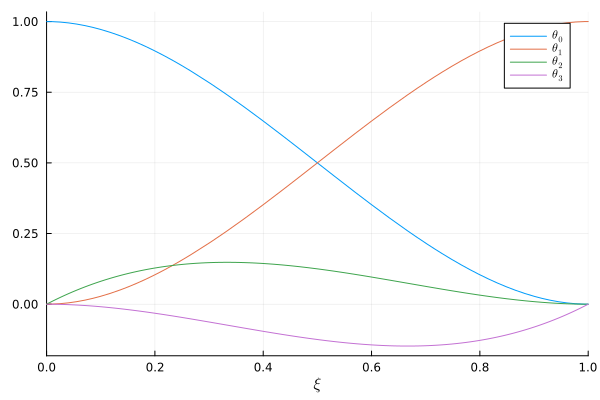
\includegraphics[width=\textwidth]{../../lectures/finite-elements/d-1/Hermite/Hermite_reference_element.png}
        \end{column}
    \end{columns}
    \medskip
    $\mathcal I_K v = v(0)\theta_0 + v(1)\theta_1 + v'(0)\theta_2 + v'(1)\theta_3$ \ matches values \emph{and} derivatives at the end points.
\end{frame}

\begin{frame}{Reference elements}
    It is convenient to do all computations on a few \alert{reference} element domains:
    \medskip
    \begin{center}
        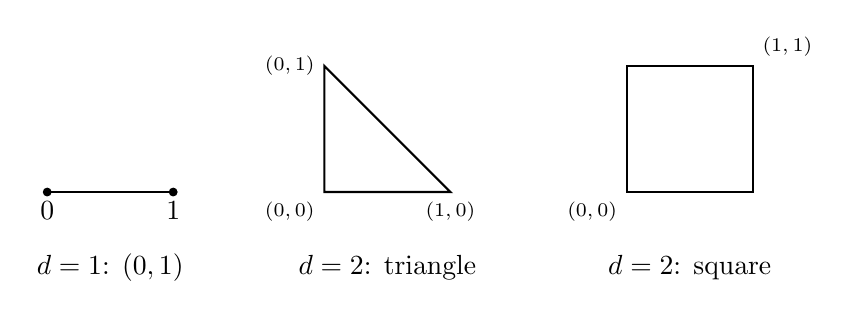
\begin{tikzpicture}[scale=1.6]
            \draw[thick] (0,0) -- (1,0);
            \fill (0,0) circle (1pt) node[below] {$0$};
            \fill (1,0) circle (1pt) node[below] {$1$};
            \node at (.5,-.6) {$d = 1$: $(0,1)$};
            \begin{scope}[xshift=2.2cm]
                \draw[thick] (0,0) -- (1,0) -- (0,1) -- cycle;
                \node[below left] at (0,0) {\scriptsize $(0,0)$};
                \node[below] at (1,0) {\scriptsize $(1,0)$};
                \node[left] at (0,1) {\scriptsize $(0,1)$};
                \node at (.5,-.6) {$d = 2$: triangle};
            \end{scope}
            \begin{scope}[xshift=4.6cm]
                \draw[thick] (0,0) rectangle (1,1);
                \node[below left] at (0,0) {\scriptsize $(0,0)$};
                \node[above right] at (1,1) {\scriptsize $(1,1)$};
                \node at (.5,-.6) {$d = 2$: square};
            \end{scope}
        \end{tikzpicture}
    \end{center}
    \medskip
    and transport them to each element of the mesh by an \alert{affine map} $F(x) = \mat A x + \vec b$.
    \takeaway{Compute once on the reference element, then change variables.}
\end{frame}

\begin{frame}{Affine equivalence}
    \begin{definition}[Affine equivalence]
        $(K,\mathcal P,\mathcal N)$ and $(\widehat K,\widehat{\mathcal P},\widehat{\mathcal N})$ are affine equivalent if there is $F(x) = \mat A x + \vec b$, $\mat A$ non-singular, such that
        \begin{enumerate}
            \item $F(K) = \widehat K$;
            \item $F^* \widehat{\mathcal P} = \mathcal P$, where $F^*\widehat v = \widehat v \circ F$ (pull-back);
            \item $F_* \mathcal N = \widehat{\mathcal N}$, where $(F_* N)(\widehat v) = N(\widehat v \circ F)$ (push-forward).
        \end{enumerate}
    \end{definition}
    \begin{example}[Linear elements in $d=1$]
        Two linear Lagrange elements on $(x_1,x_2)$ and $(\widehat x_1, \widehat x_2)$ are affine equivalent via
        \[
            F(x) = \widehat x_1 + (\widehat x_2 - \widehat x_1)\frac{x - x_1}{x_2 - x_1}.
        \]
        In particular, we can do all computations on $(0,1)$.
    \end{example}
\end{frame}

\begin{frame}{Scaling of Sobolev seminorms}
    Size of an element: \quad
    $h_K = \operatorname{diam}(K)$, \qquad $\rho_K = \sup\{\operatorname{diam}(B) : B \text{ ball contained in } K\}$.
    \begin{lemma}
        Let $F(x) = \mat A x + \vec b$, $F(K) = \widehat K$, $\widehat v \in H^m(\widehat K)$ and $v = \widehat v \circ F$. Then
        \[
            [\widehat v]_{H^m(\widehat K)} \le C\, \|\mat A^{-1}\|^m\, |\det \mat A|^{\frac 1 2}\, [v]_{H^m(K)},
            \qquad
            \|\mat A^{-1}\| \le \frac{h_K}{\rho_{\widehat K}}.
        \]
    \end{lemma}
    \begin{proofsteps}
        \begin{enumerate}
            \item Change of variables: $\int_{\widehat K} \widehat w = |\det \mat A| \int_K \widehat w \circ F$.
            \item Chain rule: each derivative produces a factor $\mat A^{-1}$.
            \item Any $\vec\xi$ with $|\vec\xi| = \rho_{\widehat K}$ is $\widehat x - \widehat y$ with $\widehat x, \widehat y \in \overline{\widehat K}$, so
                  $|\mat A^{-1}\vec\xi| = |F^{-1}\widehat x - F^{-1}\widehat y| \le h_K$.
        \end{enumerate}
    \end{proofsteps}
\end{frame}

\begin{frame}{Interpolation estimates by affine equivalence}
    \small
    \begin{theorem}
        Let $(K,\mathcal P,\mathcal N)$ (reference) and $(\widehat K,\widehat{\mathcal P},\widehat{\mathcal N})$ be affine equivalent, and assume
        \[
            [v - \mathcal I_K v]_{H^k(K)} \le C_1(K)\, [v]_{H^m(K)} \qquad \forall v \in H^m(K).
        \]
        Then
        \[
            [\widehat v - \mathcal I_{\widehat K} \widehat v]_{H^k(\widehat K)} \le C_2(K)\, \frac{h_{\widehat K}^m}{\rho_{\widehat K}^k}\, [\widehat v]_{H^m(\widehat K)},
        \]
        with $C_2$ independent of $\widehat K$.
    \end{theorem}
    \begin{proofsteps}
        \begin{enumerate}
            \item Interpolation commutes with the change of variables: $(\mathcal I_{\widehat K}\widehat v)\circ F = \mathcal I_K v$.
            \item Go to the reference element (factor $h_K^k \rho_{\widehat K}^{-k} |\det \mat A|^{\frac12}$), apply the assumption there.
            \item Come back with $F^{-1}$ (factor $h_{\widehat K}^m \rho_K^{-m} |\det\mat A|^{-\frac12}$). The determinants cancel.
        \end{enumerate}
    \end{proofsteps}
\end{frame}

\begin{frame}{A difficulty: derivatives as degrees of freedom}
    \begin{example}[Hermite cubics are not affine equivalent]
        Let $F(x) = a + (b-a)x$ map $(0,1)$ to $\widehat K = (a,b)$. Since $\frac{\diff F}{\diff x} = b - a$,
        \[
            \widehat N_1(\widehat v) = \widehat v(a),\quad
            \widehat N_2(\widehat v) = \widehat v(b),\quad
            \widehat N_3(\widehat v) = (b-a)\,\widehat v'(a),\quad
            \widehat N_4(\widehat v) = (b-a)\,\widehat v'(b).
        \]
        The natural element on $(a,b)$ uses $\widehat v'(a)$ and $\widehat v'(b)$ \alert{without} the factor $(b-a)$.
    \end{example}
    \begin{itemize}
        \item Elements with derivatives as degrees of freedom are not affine equivalent to the reference element in general.
        \item We need a more general tool: the \alert{Bramble--Hilbert lemma}.
    \end{itemize}
\end{frame}

\begin{frame}{The Bramble--Hilbert lemma}
    \begin{lemma}[Bramble--Hilbert]
        Let $\Omega \subset \R^d$ be bounded and star-shaped with respect to a ball, $m \ge 1$, $p \in (1,\infty)$.
        Let $F: W^{m,p}(\Omega) \to \R$ be linear and continuous with
        \[
            F(P) = 0 \qquad \forall P \in \R_{m-1}[x_1, \dots, x_d].
        \]
        Then $|F(v)| \le C\, \|D^m v\|_{L^p(\Omega)}$ for all $v \in W^{m,p}(\Omega)$.
    \end{lemma}
    \begin{example}[Linear interpolation in $(0,1)$]
        $E(v) = v - \big(v(0) + (v(1) - v(0))x\big)$ vanishes on $\R_1[x]$. Applying the lemma with $m = 2$:
        \[
            \|E(v)\|_{H^1(0,1)} \le C\, \|v''\|_{L^2(0,1)} .
        \]
    \end{example}
    \takeaway{If $\mathcal I_K$ reproduces polynomials of degree $m-1$, the error only sees $D^m v$.}
\end{frame}

\begin{frame}{General bound on the interpolation error}
    \begin{theorem}[Simplified statement]
        Let $(K,\mathcal P,\mathcal N)$ be a finite element such that
        \begin{enumerate}
            \item $K$ is star-shaped with respect to a ball of diameter $\rho_K$ (e.g.\ $K$ convex),
            \item $\R_{m-1}[x] \subset \mathcal P$,
            \item the nodal functions are bounded in $C^\ell(\overline K)$, with $m - \ell - \frac dp > 0$.
        \end{enumerate}
        Then, for $j = 0, \dots, m$,
        \[
            [v - \mathcal I_K v]_{W^{j,p}(K)} \le C\, h_K^{m-j}\, [v]_{W^{m,p}(K)} \qquad \forall v \in W^{m,p}(K),
        \]
        where $C$ depends on $d,m,p,\ell$, on $h_K/\rho_K$ and on $\mathcal I$ rescaled to diameter $1$.
    \end{theorem}
    \begin{proofsteps}[Idea]
        Rescale $K$ to diameter $1$, apply Bramble--Hilbert to $v - \mathcal I_K v$ (it vanishes on $\R_{m-1}$), and scale back.
    \end{proofsteps}
\end{frame}

\begin{frame}{Summary and practice}
    \begin{itemize}
        \item Finite element $= (K, \mathcal P, \mathcal N)$; nodal basis $N_i(\psi_j) = \delta_{ij}$; $\mathcal I_K v = \sum_i N_i(v)\psi_i$.
        \item Reference element $+$ affine maps: compute once, transport everywhere.
        \item Scaling: $[v - \mathcal I_K v]_{H^k} \lesssim \frac{h_K^m}{\rho_K^k}[v]_{H^m}$.
        \item Bramble--Hilbert: reproducing $\R_{m-1}$ gives order $h_K^{m-j}$.
    \end{itemize}
    \bigskip
    \textbf{Practice.} Exercises 2.1--2.4:
    \begin{itemize}
        \item 2.1: nodal basis of the Hermite cubics.
        \item 2.2: $\|v\|_{L^\infty(T)} \le C h_T^{-2} \|v\|_{L^1(T)}$ for polynomials on a triangle (go to the reference triangle).
        \item 2.3: linear element on $(a,b)$; $\mathcal I_K p = p$ for $p \in \mathcal P$.
        \item 2.4: linear Lagrange basis on a triangle; local stiffness matrix.
    \end{itemize}
    \bigskip
    \textbf{Next session:} glueing elements together.
\end{frame}
